\subsection{Geany - Entwicklungsumgebung}

Nach dem Herstellen der Verbindung zur Raspberry Pi �ber SSH, kann die grafische Entwicklungsumgebung Geany gestartet werden.

%sudo apt-get install geany xterm

\begin{console}
cd ~
geany &
\end{console}

Soll Geany in Englisch ausgef�hrt werden obwohl das System auf Deutsch gestellt wurde, so muss man vor dem Start die Variable "`LANG"' auf "`C"' setzen.

\begin{console}
LANG=C geany &
\end{console}

Nun kann eine Source-Datei geladen oder erstellt werden. Dann kann das Konfigurationsfenster ge�ffnet werden, indem man im Men� unter \texttt{Erstellen} $\rightarrow$ \texttt{Kommandos zum Erstellen konfigurieren} ausw�hlt.\\
Die Parameter f�r \texttt{Kompilieren} und \texttt{Erstellen} werden zwar bereits anhand der Source-Datei (Extention) vorbelegt. Zumeist m�ssen aber noch Anpassungen vorgenommen werden, um Bibliotheken oder ge�nderte Kompiler verwenden zu k�nnen. Was genau hier einzutragen ist, wird in den folgenden Beispielprogrammen der einzelnen Programmiersprachen angegeben.\\  
Danach kann das Programm mit der Taste \texttt{Erstellen} erzeugt werden und mit der Taste \texttt{Ausf�hren} auch in einem Terminal gestartet werden.\\
Die Tastenk�rzel f�r alle Funktionen k�nnen �ber das Men� \texttt{Bearbeiten} $\rightarrow$ \texttt{Einstellungen} $\rightarrow$ \texttt{Tastenk�rzel} vorgegeben werden. Dazu w�hlt man die gew�nschte Aktion aus und dr�ckt die Taste "`�ndern"'. Danach kann man die Taste bzw. Tastenkombination dr�cken, die dann umgehend im Dialog angezeigt wird. Wenn nun die OK-Taste gedr�ckt wird, wird die �nderung �bernommen und das Tastenk�rzel f�hrt in Zukunft die Aktion aus. 
Im Beispiel wurde der Aktion "`Erstellen"' dem Tastenk�rzel bzw. der Taste \framebox{F7} zugewiesen. 

%\begin{figure}[ht]
%  \centering
%  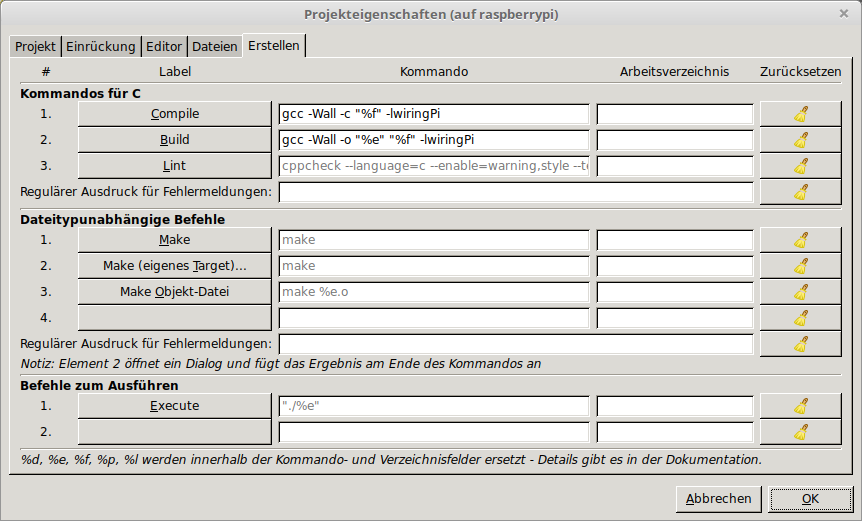
\includegraphics[scale=0.48]{images/Geany_Create.png}
%  \caption{Kommandos zum Erstellen konfigurieren f�r C Projekt}
%  \label{Geany-create}
%\end{figure}

\begin{figure}[ht]
  \centering
  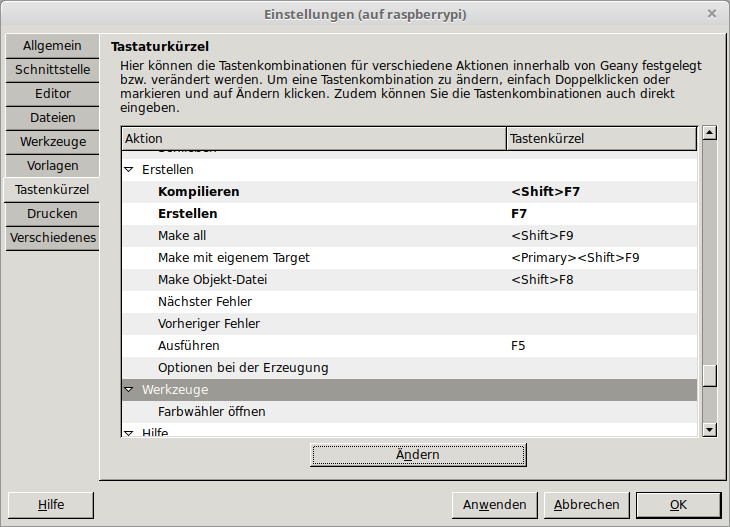
\includegraphics[scale=0.48]{images/Geany_Settings.png}
  \caption{Tastaturk�rzel}
  \label{Geany-settings}
\end{figure} 

\begin{figure}[ht]
  \centering
  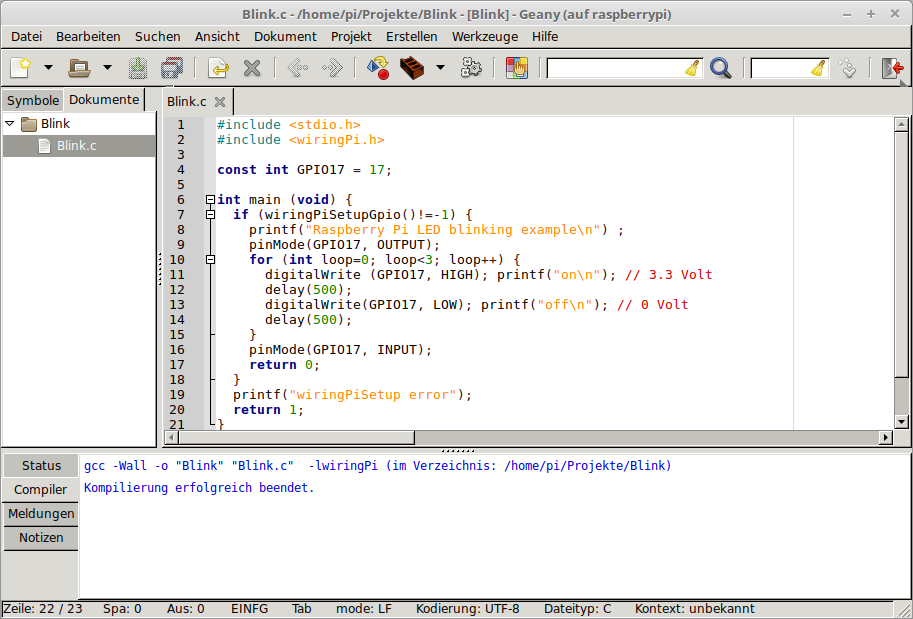
\includegraphics[scale=0.4]{images/Geany_Window.png}
  \caption{Geany Oberfl�che mit Blink-LED Beispiel}
  \label{Geany-window}
\end{figure}
